\documentclass{beamer}

% Top-aligning columns within a top-aligned frame
% https://tex.stackexchange.com/questions/16447/beamer-top-aligning-columns-within-a-top-aligned-frame
\makeatletter
\newenvironment{myitemize}{%
   \setlength{\topsep}{0pt}
   \setlength{\partopsep}{0pt}
   \renewcommand*{\@listi}{\leftmargin\leftmargini \parsep\z@ \topsep\z@ \itemsep\z@}
   \let\@listI\@listi
   \itemize
}{\enditemize}
\makeatother  

\usepackage[USenglish]{babel}
\usepackage[utf8]{inputenc}
\usepackage{amssymb, amsmath}
\usepackage{bm}
\usepackage{color}
\usepackage{tikz}
\usepackage{url}
%\usepackage{algpseudocode}
\usepackage[ruled,vlined]{algorithm2e}
%\usepackage{algorithm,algorithmic}


\definecolor{links}{HTML}{2A1B81}
\hypersetup{colorlinks,linkcolor=,urlcolor=links}

\usetheme{Boadilla}
\setbeamertemplate{headline}{}
\newcommand*\oldmacro{}%
\let\oldmacro\insertshorttitle%
\renewcommand*\insertshorttitle{%
  \oldmacro\hfill%
  \insertframenumber\,/\,\inserttotalframenumber}
  

\bibliographystyle{apalike}
% make bibliography entries smaller
%\renewcommand\bibfont{\scriptsize}
% Now get rid of all the colours
\setbeamercolor*{bibliography entry title}{fg=black}
\setbeamercolor*{bibliography entry author}{fg=black}
\setbeamercolor*{bibliography entry location}{fg=black}
\setbeamercolor*{bibliography entry note}{fg=black}

\newcommand{\lnorm}[1]{\left\lVert#1\right\rVert^2}
\newcommand{\norm}[1]{\left\lVert#1\right\rVert}

% and kill the abominable icon
\setbeamertemplate{bibliography item}{}

\begin{document}
\title{Adam}  
\author{Radek Bartyzal}
\date{TBD} 
\institute{MI-SZI}

\frame{\titlepage} 

\begin{frame}{Training of neural nets}
\onslide<1->{
\begin{block}{Goal}
Set weights $w$ and biases $b$ in such way that the network approximates the desired outputs $y(x)$ for every input $x$.
\end{block}
}

\onslide<2->{
How to get there?
\begin{enumerate}
\item choose a function that tells you the error of the network
 = cost function
\item minimize the cost function
\end{enumerate}
}

\onslide<3->{
\begin{block}{Cost function}
Quantifies how well the network approximates the desired outputs $y(x)$ for every input $x$. 
\end{block}
}

\end{frame}


\begin{frame}{Training 1: Cost function}

%\begin{block}{Cost function}
= loss function = objective function. \\
Quantifies how well the network approximates the desired outputs $y(x)$ for every input $x$. 
%\end{block}

\begin{block}{Mean Squared Error (MSE)}
\begin{tabbing}
$w$ = weights \hspace{40mm} \= $b$ = biases\\
$n$ = number of inputs \> $x$ = one input\\
$a$ = output of network for $x$\\
$y(x)$ = desired output for $x$
\end{tabbing}
$$
C(w,b) = \frac{1}{2n} \sum_x{ \| y(x) - a \|^2}
$$
\end{block}
\end{frame}


\begin{frame}{Training 1: Cost function}
Our goal is to minimize the cost function = move $w$ and $b$ in a direction that lowers the value of the cost function.
\vfill
\begin{block}{Why Mean Squared Error ?}
\begin{itemize}
\item \textbf{smooth function of weights and biases} - even small changes of $w$ or $b$ result in a change of the function value
\item \textbf{easily derivable} - we need derivation of the cost function to calculate the direction in which we should change the $w$ and $b$
\end{itemize}
\end{block}
\end{frame}


\begin{frame}{Training 2: Gradient descent}
\onslide<1->{
\begin{block}{Gradient}
Vector = direction in which the function increases the most in value.
\end{block}
}

\onslide<2->{
\begin{block}{Gradient descent}
\begin{enumerate}
\item calculate gradient of the cost function
\item take step in opposite direction = change $w$ and $b$ in a way that lowers the value of the cost function
\end{enumerate}
\end{block}
}

\onslide<3->{
\begin{block}{Learning rate = $\eta$}
How large is the step we take.
\end{block}
}
\end{frame}


\begin{frame}{Training 3: Backpropagation}

\begin{block}{Backpropagation algorithm}
Efficient way of calculating the gradient of the cost function with respect to any neuron = to any weight or bias.
\end{block}
\vfill
Tells us in which direction should we move the weights and biases to reduce the error.
\vfill
Works by propagating the error back from the output layer to the input layer.
\end{frame}

\begin{frame}{Mini-Batch Gradient Descent}

\begin{algorithm}[H]
  \label{alg:mini_SGD}
  \caption{Mini-batch Stochastic Gradient Descent}
  \DontPrintSemicolon
  $\theta = \theta_0$\;
  \For{$t\gets 1$ \KwTo $T$}
  {
  $\mathit{shuffle(dataset)}$\;
  \ForEach{$\text{mini\_batch} \in \text{dataset}$}
  {
  $g = 0$\;
  \ForEach{$i \in \text{mini\_batch}$}
    {
     $g = g + \nabla L(\hat{y}_i,f(\theta, x_i))$\;
    }
  $g = \frac{1}{B} g$\;
  $\theta = \theta - \eta g$
  }
  }
\end{algorithm}

\end{frame}
%--------- END Frame 1 -------------

\begin{frame}{Visualization of Gradient Descent}

\begin{figure}[h]
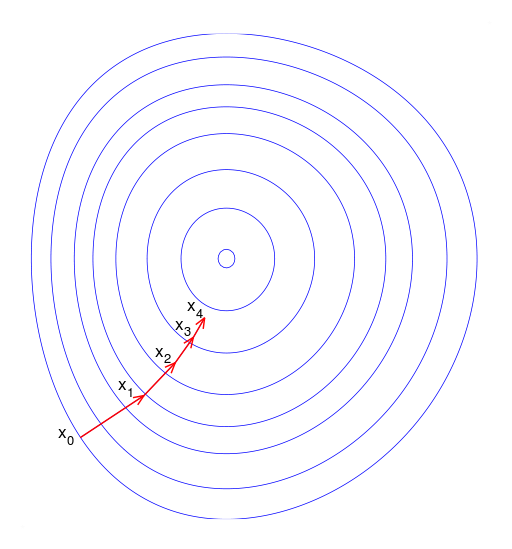
\includegraphics[scale=0.4]{img/nice_space}
\end{figure}

\end{frame}
%--------- END Frame 1 -------------

\begin{frame}{More realistic space}

\begin{figure}[h]
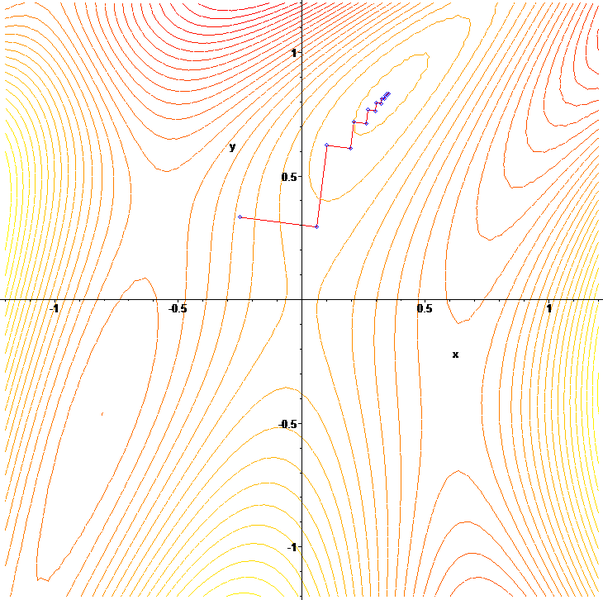
\includegraphics[scale=0.35]{img/real_space}
\end{figure}

\end{frame}
%--------- END Frame 2 -------------
\begin{frame}{Saddle point}

\begin{figure}[h]
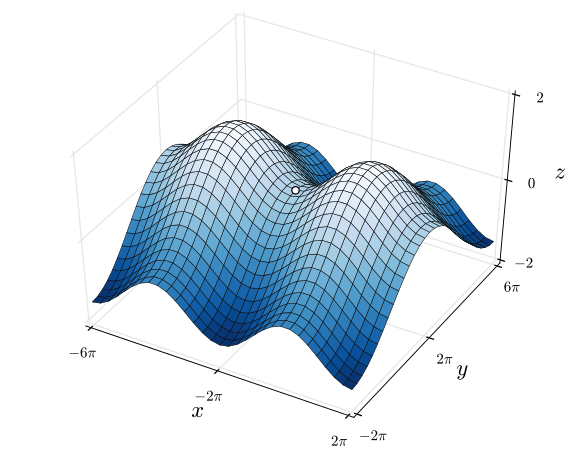
\includegraphics[scale=0.55]{img/saddle}
\end{figure}

\end{frame}
%--------- END Frame 2 -------------
\begin{frame}{Rosenbrock function = long descending valley}

\begin{figure}[h]
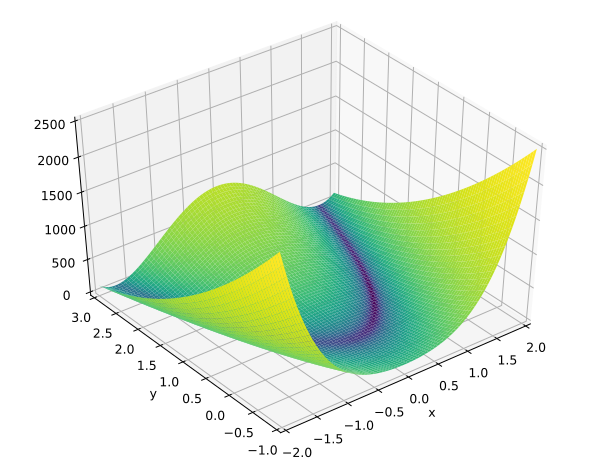
\includegraphics[scale=0.50]{img/rosenbrock_function}
\end{figure}

\end{frame}
%--------- END Frame 2 -------------
\begin{frame}{Problems of SGD}

\begin{itemize}
\item same learning rate for each parameter $\implies$ Adaptive Gradient:
\begin{equation}\label{eq:adagrad_update}
\theta_{t+1,i}^{AdaGrad} = \theta_{t,i} - \frac{\eta}{\sqrt{ \sum_{\tau=1}^t{g_{\tau,i}^2}} + \epsilon} g_{t,i}
\end{equation}

\item slow traversal of saddle points $\implies$ momentum \cite{cit:ruder}:
\begin{align}
\begin{split}
g_t &= \gamma g_{t-1} + \eta \nabla_\theta L( \theta) \\  
\theta &= \theta - g_t
\end{split}
\end{align}

\end{itemize}

\end{frame}
%--------- END Frame 2 -------------
\begin{frame}{Momentum}

\begin{figure}[h]
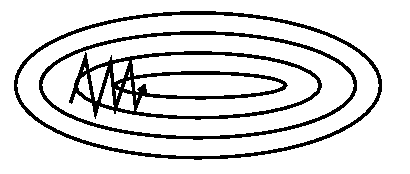
\includegraphics[scale=0.70]{img/without_momentum}
\caption{Without momentum \cite{cit:ruder}.}
\end{figure}

\begin{figure}[h]
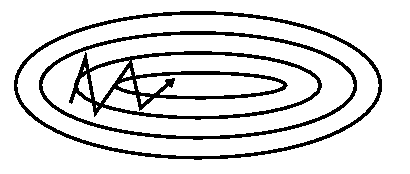
\includegraphics[scale=0.70]{img/with_momentum}
\caption{With momentum \cite{cit:ruder}.}
\end{figure}

\end{frame}
%--------- END Frame 2 -------------
\begin{frame}{Adam}
First and second order moments:
\begin{equation}\label{eq:adam_moments}
\begin{aligned}
m_t &= \beta_1 m_{t-1} + (1 - \beta_1) g_t\\
v_t &= \beta_2 v_{t-1} + (1 - \beta_2) g_t^2
\end{aligned}
\end{equation}

Bias corrected:
\begin{equation}\label{eq:adam_moments}
\begin{aligned}
\hat{m_t} &= \frac{m_t}{(1 - \beta_1^t)}\\
\hat{v_t} &= \frac{v_t}{(1 - \beta_2^t)}
\end{aligned}
\end{equation}

Parameter update:
\begin{equation}\label{eq:adam_update}
\theta_{t+1}^{Adam} = \theta_{t} - \frac{\eta}{\sqrt{v_t} + \epsilon} m_t
\end{equation}

\end{frame}
%--------- END Frame 2 -------------

%--------- END Frame 12 -------------
\begin{frame}{Sources}

\begin{thebibliography}{0}

  \bibitem[1]{cit:ruder} 1. Ruder, Sebastian. "An overview of gradient descent optimization algorithms." arXiv preprint arXiv:1609.04747 (2016).
  
\end{thebibliography}

\end{frame}

 
 
 
\end{document}
